\chapter{Fachliche Grundlagen}
In diesem Kapitel werden \gls{hl} bezogene fachliche Grundlagen erläutert. Dies ist notwendig, um die Problemstellung sowie Teile der internen Strukturen zu verstehen.

\section{Wie kommt eine Buchung auf die Waitinglist}
Um zu verstehen, wann die Waitinglist zum Einsatz kommt, muss zunächst eine Wissensgrundlage des Prozesses der Buchung eines Transports bei \gls{hl} geschaffen werden.
%%%%%%%%%%%%%%%%%%%%%%%%%%%%%%%%%%%%%%%%%%%%%
\subsection{Buchung}
%\todo{IW: Waitinglist erklären}
%Entscheidendes Manko: Sie erklären hier die Terme Buchung, Transport Unit Point und Announcement, aber leider nicht Waitinglist.
%Beim Transport bei einer Reederei hingegen unterscheidet sich dieser Prozess deutlich

Ein Transport bei einer Reederei weist in gewissen Aspekten Ähnlichkeiten zur Nutzung öffentlicher Verkehrsmittel auf. 
Bei einem Transport mit den öffentlichen Verkehrsmitteln zwischen zwei Punkten wird in der Regel ein Buchungsportal oder ein Fahrkartenschalter genutzt. 
Dabei gibt man den Start- und Zielpunkt sowie das gewünschte Datum für die Reise an. Anschließend erhält der Kunde Vorschläge für verfügbare Optionen, aus denen gewählt werden kann.

Der Buchungsprozess bei einer Reederei unterscheidet sich wie folgt von diesem Vorgehen:
Zunächst stellt ein Kunde, i.d.R. eine Firma, eine Anfrage an eine Reederei. 
Die Anfrage muss mindestens Ausgangspunkt und Ziel sowie ein gewolltes Ankunftsdatum enthalten. 
Es kann aber auch vom Kunden eine Route vorgegeben werden, um bestimmte Schiffe zu vermeiden oder Verzögerungen zu umgehen.
Die Reederei beantwortet dies mit einem Angebot, welches einen voraussichtlichen Preis, eine konkrete Route und die Information darüber, wie lange das Angebot gültig ist, enthält. Dieses wird auch die \gls{quote} genannt. 

Es gibt unterschiedliche Arten von \glspl{quote}. Eine Spot-\gls{quote} bedeutet, dass das Angebot nur für eine bestimmte Abfahrt und Route gültig ist \cite{hapaglloyd_quick_quotes}, ähnlich wie eine Zugbindung im öffentlichen Verkehr. Im Gegensatz dazu sind klassische \glspl{quote} ohne eine bestimmte Abfahrt und daher meist mehrere Wochen bis Monate gültig.

Diese \gls{quote} kann der Kunde prüfen und bei Zustimmung annehmen. 
Wenn der Kunde eine \gls{quote} annimmt, wird eine Buchung in dem internen System erstellt (auch \enquote{Shipment} genannt), in der alle bis jetzt bekannten Daten gesammelt werden. 

Es ist noch wichtig zu beachten, dass bei einer Buchung zwei unterschiedliche Kunden involviert sein können. Einerseits gibt es den \enquote{Endkunden}, für den der Container letztlich geliefert wird und andererseits, den \enquote{vertraglichen Kunden}, mit dem die Reederei direkt den Vertrag schließt. 
In vielen Fällen handelt es sich hierbei um denselben Kunden. Es kann jedoch auch sein, dass der Endkunde eine Spedition beauftragt, die wiederum die Reederei für den Transport engagiert. In diesem Fall steht die Reederei im direkten Vertragsverhältnis mit der Spedition, während die tatsächliche Lieferung für den Endkunden erfolgt.


%%%%%%%%%%%%%%%%%%%%%%%%%%%%%%%%%%%%%%%%%%%%%
\subsection{Transport Unit Point}
 Innerhalb einer Buchung gibt es einzelne \glspl{tup}. Ein \gls{tup} ist ein Abschnitt der Strecke, bestehend aus einem Startpunkt, einem Zielpunkt und dem dazugehörigen Transport. Wichtig ist dabei, dass sich ein \gls{tup} immer nur auf eine einzelne zu transportierende Einheit (\acrshort{tu}\glsunset{tu}) bezieht, also beispielsweise einen spezifischen Container oder ein Flugzeugteil. Das bedeutet, dass für jede Einheit in einer Lieferung ein eigener \gls{tup} geplant wird.

Um dies zu verdeutlichen, nehmen wir das Beispiel eines Containers, der von einer Firma in Wedel zu einer Firma in Singapur geliefert wird. Der Transport beginnt in Wedel, von wo aus der Container zunächst mit einem LKW zum Hamburger Hafen gebracht wird. Anschließend wird der Container per Schiff nach Singapur transportiert, bevor er schließlich von dort mit einem weiteren LKW zur Firma in Singapur geliefert wird.

\pagebreak
Die gesamte Lieferstrecke kann somit in die folgenden \glspl{tup} unterteilt werden:
\begin{itemize}[noitemsep]
    \item Firmenstandort in Wedel: Transport eines Containers mit einem LKW zum Hamburger Hafen.
    \item Hamburger Hafen: Verschiffung des Containers nach Singapur.
    \item Hafen in Singapur: Transport des Containers mit einem LKW zur Firma in Singapur.
    \item Firmenstandort in Singapur: Endpunkt, da keine weitere Folgeposition definiert ist.
\end{itemize}

Ein wichtiger Bestandteil der Planung eines \gls{tup} ist das eingesetzte Transportmittel. Im Fall des maritimen Transports kommen Schiffssysteme und sogenannte \glspl{dpvoyage} zum Einsatz. Ein Schiffssystem lässt sich mit einer U-Bahn-Linie vergleichen: Es handelt sich um eine feste Route, die regelmäßig von Schiffen bedient wird, ähnlich wie eine U-Bahn, die bestimmte Haltestellen in festgelegten Abständen anfährt. Eine \gls{dpvoyage} ist dabei vergleichbar mit einer einzelnen Bahn auf dieser Strecke, die zu einem bestimmten Zeitpunkt fährt. Allerdings muss eine \gls{dpvoyage} nicht zwingend jede Station des Schiffssystems ansteuern. Beispielsweise kann ein Schiff im Rahmen einer \gls{dpvoyage} nur die Häfen Hamburg und Singapur anlaufen und Rotterdam auslassen, wenn dort keine Ladung zu entladen oder aufzunehmen ist.

Die Kombination aller \glspl{tup} ergibt die vollständige Lieferkette. Für jeden \gls{tup} wird der Transport separat geplant, einschließlich der eingesetzten Transportmittel. Dabei wird festgelegt, welches Transportmittel verwendet wird.
Beispielsweise wird auf dem Abschnitt zwischen dem Hamburger Hafen und Singapur ein bestimmtes Schiff im Rahmen einer \gls{dpvoyage} eingeplant, während die anderen Abschnitte mit LKWs oder anderen passenden Transportmitteln durchgeführt werden.

%%%%%%%%%%%%%%%%%%%%%%%%%%%%%%%%%%%%%%%%%%%%%
\subsection{Announcements}
\label{ref:announcement}

%\todo{IW: Spätestens hier muss die waitinglist erklärt sein!}
%

Die bis hierhin gesammelten Informationen müssen nun der operativen Seite zur Überprüfung übermittelt werden.
%Die bis hierhin gesammelten Daten sind zunächst nur für die Planung, wie die einzelnen \glspl{tu} transportiert werden sollen. Die operative Seite hat zu diesem Zeitpunkt noch keine Informationen darüber erhalten. 
Die operative Seite umfasst alle Beteiligten, die für die tatsächliche Durchführung des Transports notwendig sind, wie Häfen, Containerdepots, Schiffe und andere Ressourcen. Daher muss die interne Bestellung nun mit der operativen Seite abgestimmt werden, um sicherzustellen, dass die Buchung so wie geplant überhaupt umsetzbar ist. Für diese Abstimmung wird der Announcement-Prozess eingeleitet, bei dem versucht wird, die einzelnen \glspl{tup} in die operative Welt zu überführen. Es werden zunächst Konsistenzchecks durchgeführt. Es wird also überprüft, ob alle benötigten Daten vorhanden sind. 

%Auf diese Checks wird nicht weiter drauf eingegangen, da sie erstmals nicht für die Waitinglist relevant sind.
Folgende Grafik veranschaulicht einen Teil des Announcement-Prozesses, der entscheidet, ob ein \gls{tup} angenommen, abgelehnt oder auf der Waitinglist landet:

\begin{figure}[H]
    \centering
    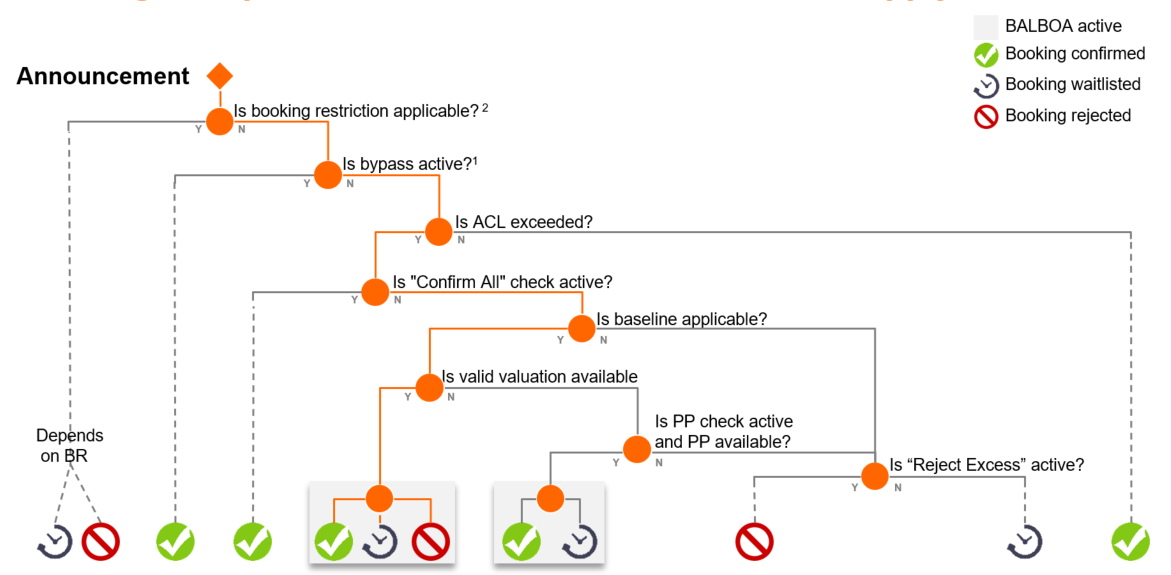
\includegraphics[width=0.8\textwidth]{bilder/waitling_checks.png}
    \caption
    [Teil des Announcement-Prozesses] % Text, der im Bildverzeichnis verwendet wird
    {Teil des Announcement-Prozesses \cite{baselined_booking_acceptance}} % Quelle Hinzufügen
    \label{fig:ann_process}
\end{figure}

Für jeden \gls{tup} wird dieser Announcement-Prozess durchlaufen. 
Er beginnt mit der Prüfung auf Buchungsrestriktionen. 
Eine Buchungsrestriktion ist eine Art Filter, der auf verschiedenen Kriterien basiert. 
Wenn eine Restriktion greift, entscheidet die Regel darüber, ob die Buchung für den \gls{tup} abgelehnt oder auf die Waitinglist gesetzt wird. 
Dies wurde beispielsweise eingesetzt, als im Jahr 2023 Schiffe von \gls{hl} im Roten Meer angegriffen wurden, um zu verhindern, dass Schiffe an dieser Position entlangfahren.
Also wurden alle \glspl{tup}, welche dort entlangfahren sollten, abgelehnt.
Die Restriktionen können aber auch so eingestellt werden, dass Buchungen nicht abgelehnt, sondern auf die Waitinglist geschrieben werden.
%\todo{IW: Was hat mit Warten zu tun?}
%Hier ist mir unklar, was das mit Warten zu tun hat: Wenn eine Route gar nicht befahrbar ist, dann kann man sie  überhaupt nicht buchen. Und wenn ich Ihre U-Bahn-Analogie benutze: Normalerweise will ich vom Informationsanbieter nur wissen, wie ich im Moment schnellstmöglich (oder am kostengünstigsten) von A nach B komme, und da mache ich keine Vorgaben, welche Route genommen werden soll. Das ist dann ein internes Problem für den Informationsanbieter, und der muss mir keinen Grund nennen, warum eine bestimmte Route (die ich als Fragesteller ja vielleicht gar nicht kenne) gerade nicht funktioniert. Der Fragesteller erwartet vom Informationsanbieter lediglich, dass dessen Auskünfte zuverlässig sind.

Falls keine Buchungsrestriktion greift, wird geprüft, ob der \enquote{Bypass} aktiviert ist. Dieser wird beispielsweise bei einer Spot-Buchung verwendet, also einer Buchung mit Mitnahmegarantie. Ist dies der Fall, wird die Buchung direkt bestätigt, ohne weitere Prüfungen durchzuführen. Liegt kein \enquote{Bypass} vor, geht der Prozess weiter mit der Überprüfung des \gls{acl}.

Das \gls{acl} ist das vertraglich festgelegte Volumen, das pro Kunde automatisch akzeptiert wird. Wenn das verfügbare \gls{acl} nicht überschritten wurde, wird die Buchung automatisch bestätigt. Falls jedoch das \gls{acl} überschritten ist, wird als nächstes geprüft, ob bei dem Kunden die \enquote{Confirm All}-Option aktiviert ist. Ist dies der Fall, wird die Buchung trotz überschrittenem \gls{acl} akzeptiert.

Wenn die \enquote{Confirm All}-Option nicht aktiv ist, wird die Buchung weiter geprüft. Hierbei wird der Wert der Buchung betrachtet, und es wird analysiert, ob eine Baseline anwendbar ist. Baselines sind finanzielle Schwellenwerte, die festlegen, ob eine Buchung angenommen, abgelehnt oder auf die Waitinglist gesetzt wird. Für die Bewertung wird entweder der aktuelle \hyperref[ref:balboa]{\gls{balboa}-Wert} oder, falls kein solcher Wert vorhanden ist und es zugelassen wird, der sogenannte \enquote{Past Performance}-Wert der Buchung verwendet.  
Dabei werden die vergangenen Werte des Kunden herangezogen, um auf die aktuelle finanzielle Leistung zu schließen.  
Wenn diese Bedingungen nicht erfüllt sind, kommt die \enquote{Reject Excess}-Regel zur Anwendung.

Diese Regel führt dazu, dass Buchungen, die das \gls{acl}-Volumen überschreiten, abgelehnt werden, anstatt auf die Waitinglist gesetzt zu werden.

In diesem Prozess können also \glspl{tup}, beziehungsweise \glspl{tu} für eine bestimmte Schiffsstrecke, auf der Waitinglist landen. Somit ist die Waitinglist Teil des Announcement-Prozesses.
%\todo{IW: Fragesteller (Siehe Kommentar)}
%Das wirkt hier so, als ob der Fragesteller schon die Route vorgibt (warum eigentlich?) und dass es ein großes Problem sein kann, einen Platz dort zu bekommen. Das sollten Sie genauer motivieren (falls es so ist) oder den Prozess genauer erklären (falls es nicht so ist). Jedenfalls sollten Sie genau erklären, was eine Waitinglist ist und wozu man die benutzt.
%Ausgehend von dem U-Bahn-Beispiel hätte ich gesagt: "Mir ist doch egal, ob die U-Bahn fährt oder nicht: Gib mir einfach die beste Verbindung, die gegenwärtig möglich ist. Ich nehme notfalls auch den Bus."
%Auf den Container übertragen heißt das: Wenn der Container im Moment besser um das Kap der Guten Hoffnung fahren soll als durchs Rote Meer, dann sei es so. Interessant könnte hier natürlich eine Abwägung der Kosten, Fahrzeit und Sicherheit sein, welche vermutlich gegenläufig sind.

%%%%%%%%%%%%%%%%%%%%%%%%%%%%%%%%%%%%%%%%%%%%%
\subsection{Valuations (Balboa)}
\label{ref:balboa}
Die \gls{balboa} wird eingesetzt, wenn während eines \hyperref[ref:announcement]{Annoucments} das verfügbare Kontingent überschritten wird. 
Dabei handelt es sich um das Volumen (\gls{acl}), das mit Kunden in Verträgen festgelegt wird, um freie Kontingente auf bestimmten Strecken zu sichern.  

%\todo{IW: Warum kann ein Kontingent überschritten werden? Welches Kontingent meinen Sie?}

Um dies zu erreichen, vergleicht \gls{balboa} das \acrlong{cl} 2 (\acrshort{cl}2) oder das \gls{icl} der angekündigten Buchung mit den in den Baselines vordefinierten Grenzwerten. 
Die \gls{cl} sind ein Konzept, um zu bestimmen, wie viel ein Transport beiträgt, die Kosten von \gls{hl} zu decken.
Es gibt dabei \gls{cl}1 bis \gls{cl}4 und dazu das \gls{icl}.

Die \acrlong{cl} sind gestaffelt aufgebaut. 

\begin{table}[H]
    \centering
    \begin{tabular}{p{1cm}p{14cm}}
        \hline\hline
         \multicolumn{2}{l}{\textbf{Umsatz} (alle Einnahmen im Zusammenhang mit dem Transport)} \\ \hline
         - & Variable oder direkte Kosten: Sie existieren nicht, wenn der Transport nicht stattfindet (z.B. Kosten für das Be- und Entladen von Containern). \\
         \multicolumn{2}{l}{ $\implyarrow$ \textbf{\gls{cl}1} (Teil der Einnahmen, der noch indirekte und fixe Kosten deckt)} \\ \hline
         - & Indirekte Kosten: Nicht direkt durch einen bestimmten Transport verursacht, aber durch den individuellen Transport beeinflusst (z.B. Verwaltungs- und Personalkosten). \\
         \multicolumn{2}{l}{ $\implyarrow$ \textbf{\gls{cl}2} (Teil der Einnahmen, der noch fixe Kosten deckt)} \\ \hline
         - & Betriebliche Fixkosten: Kosten für die Bereitstellung und den Betrieb der Schiffe (z.B. Kosten für Wartung und Instandhaltung). \\
         \multicolumn{2}{l}{ $\implyarrow$ \textbf{\gls{cl}3} (Teil der Einnahmen, der nach Abzug der betrieblichen Fixkosten verbleibt)} \\ \hline
         - & Weitere Fixkosten: Sie ändern sich nicht, abhängig davon, ob mehr oder weniger Transporte stattfinden. (z.B. Mietkosten für Büroräume) \\
         \multicolumn{2}{l}{ $\implyarrow$ \textbf{\gls{cl}4} (Teil der Einnahmen, der nach Abzug aller Kosten verbleibt)} \\ \hline\hline
    \end{tabular}
    \caption{\acrlong{cl} Staffelung}
    \label{tab:cl_table}
\end{table}

In der \cref{tab:cl_table} zeigt sich: Je höher das \gls{cl}, umso mehr Kosten werden vom Umsatz abgezogen.
Das \gls{icl} basiert wie das \gls{cl}2 auf dem \gls{cl}1. Der Unterschied ist aber, dass die Kosten für die Ausgleichsbewegungen von Containern zwischen verschiedenen Standorten pro Container eingerechnet werden. 

Durch den \gls{icl} kann ein Transport auch dann als profitabel bewertet werden, wenn der Preis unter den reinen variablen Kosten liegt, da die Ausgleichskosten in die Berechnung einfließen.

Als Beispiel für die Ausgleichskosten kann die Situation zwischen Europa und Asien gesehen werden. 
Es werden viele Container von Asien nach Europa transportiert, aber wenig zurück von Europa nach Asien. 
Das bedeutet, dass sich auf Dauer mehr Container in Europa sammeln und in Asien ein Mangel aufgebaut wird. 
Aufgrund dieses Mangels müssen leere Container nach Asien verschifft werden. Diese Kosten müssen rein durch \gls{hl} getragen werden und werden als Ausgleichskosten bezeichnet. Für \gls{hl} kann es daher wirtschaftlich sinnvoll sein, einen Container zu einem reduzierten Preis anzubieten, sofern die dadurch entstehenden Einnahmen die ohnehin anfallenden Kosten für den Ausgleich des Containergleichgewichts zumindest teilweise decken.

%\todo{IW: Sie sollten diese Contribution Levels beschreiben: Was ist das, was machen die und warum gibt es sie?}


%\todo{IW: Ausgleichkskosten erklären}
%Hier fehlt dem Leser die Info, für wen diese Ausgleichskosten (die hier das erste Mal erwähnt werden) relevant sind. Wieder sollte erklärt werden: Was, wie genau und warum?

Für jede Baseline können entweder Bestätigungs- oder Ablehnungsgrenzwerte definiert werden – oder beides. Wird der Bestätigungsgrenzwert überschritten, wird die Buchung automatisch bestätigt. Wird der Ablehnungsgrenzwert nicht erreicht, wird die Buchung abgelehnt. In allen anderen Fällen setzt \gls{balboa} die Buchung standardmäßig auf die Waitinglist.

In der Praxis wird für die meisten (>96 \%) Baselines das \gls{cl}2 verwendet, da es eine schnelle und effiziente Methode ist, um die Profitabilität von Buchungen zu bewerten. Das \gls{icl} wird in spezifischen Fällen herangezogen, wenn zusätzliche Kostenfaktoren durch Container-Ungleichgewichte berücksichtigt werden müssen.

%%%%%%%%%%%%%%%%%%%%%%%%%%%%%%%%%%%%%%%%%%%%%
\subsection{Waitinglist}
% Unterschied Area und Operational Waitinglist 
%\todo{IW: Waitinglist erklären}
%Der geforderte Abschnitt ist zwar da, aber Sie setzen die Kenntnis einer Waitinglist schon vorher voraus, und auch hier erklären Sie das nicht grundlegend. Es mag ja sein, dass man die hier geschilderten Eigenschaften einer Waitinglist auch verstehen sollte, aber dazu muss man erst mal verstehen, was eine Waitinglist ist.
%Eigenkommentar: Er findet, dass nicht gesagt wurde was eine Waritinglist.. also mit annahme und ablehung etc


%Wie in \sref{ref:announcement} beschrieben kann eine Buchung auf der Waitinglist landen. 

Wie erläutert handelt es sich bei der Waitinglist, um eine Warteliste, auf der ein \gls{tup} von einer Buchung landen kann. 
Die Aufnahme in die Waitinglist erfolgt im Announcement-Prozess entweder aufgrund manueller Regeln (Buchungsrestriktionen), eines aufgebrauchten Vertragsvolumens (\gls{acl}) oder aufgrund mangelnder Rentabilität (\gls{cl}).
Damit eine Buchung weiter verarbeitet und von der Waitinglist entfernt wird, muss diese entweder von der Waitinglist \textit{\textbf{akzeptiert}} oder \textit{\textbf{abgelehnt}} werden. 
Eine Ablehnung führt dabei nicht zwangsläufig zur Stornierung der Buchung, sondern erfordert die Suche nach einer alternativen Transportmöglichkeit, beispielsweise auf einem anderen Schiff.
Auch hierbei muss der Announcement-Prozess wieder durchlaufen werden und die Buchung kann erneut auf der Waitinglist landen.

Dabei muss aber unterschieden werden, ob eine Buchung, auf der Area- oder der Operational-Waitinglist landet. Der Unterschied besteht darin, dass die Operational-Waitinglist sich um operationelle Restriktionen bezieht, welche von dem Carrier bestätigt werden muss. Das wäre beispielsweise eine \gls{oog} Lieferung.
Bei \gls{oog} Lieferungen werden \glspl{tu} transportiert, welche nicht in einen normalen Containerslot passen. Diese müssen vom Carrier bestätigt werden. 

% Wir nehmen Areawaitinglist
Der Fokus dieser Arbeit liegt auf der Area-Waitinglist, denn diese behandelt das Thema, wie viele Lieferungen noch auf ein Schiff gelangen sollen.

% Wie wird aktuell die Waitinglist verarbeitet?
Die Area-Waitinglist wird von den jeweiligen Regionen manuell über den \enquote{A1050-Screen} bearbeitet. \enquote{Screens} sind grafische Oberflächen, die im firmeninternen \gls{fis}-Framework erstellt und darüber auch angezeigt werden können. 
Der \enquote{A1050-Screen} sieht wie folgt aus:

% A1050
\begin{figure}[H]
    \centering
    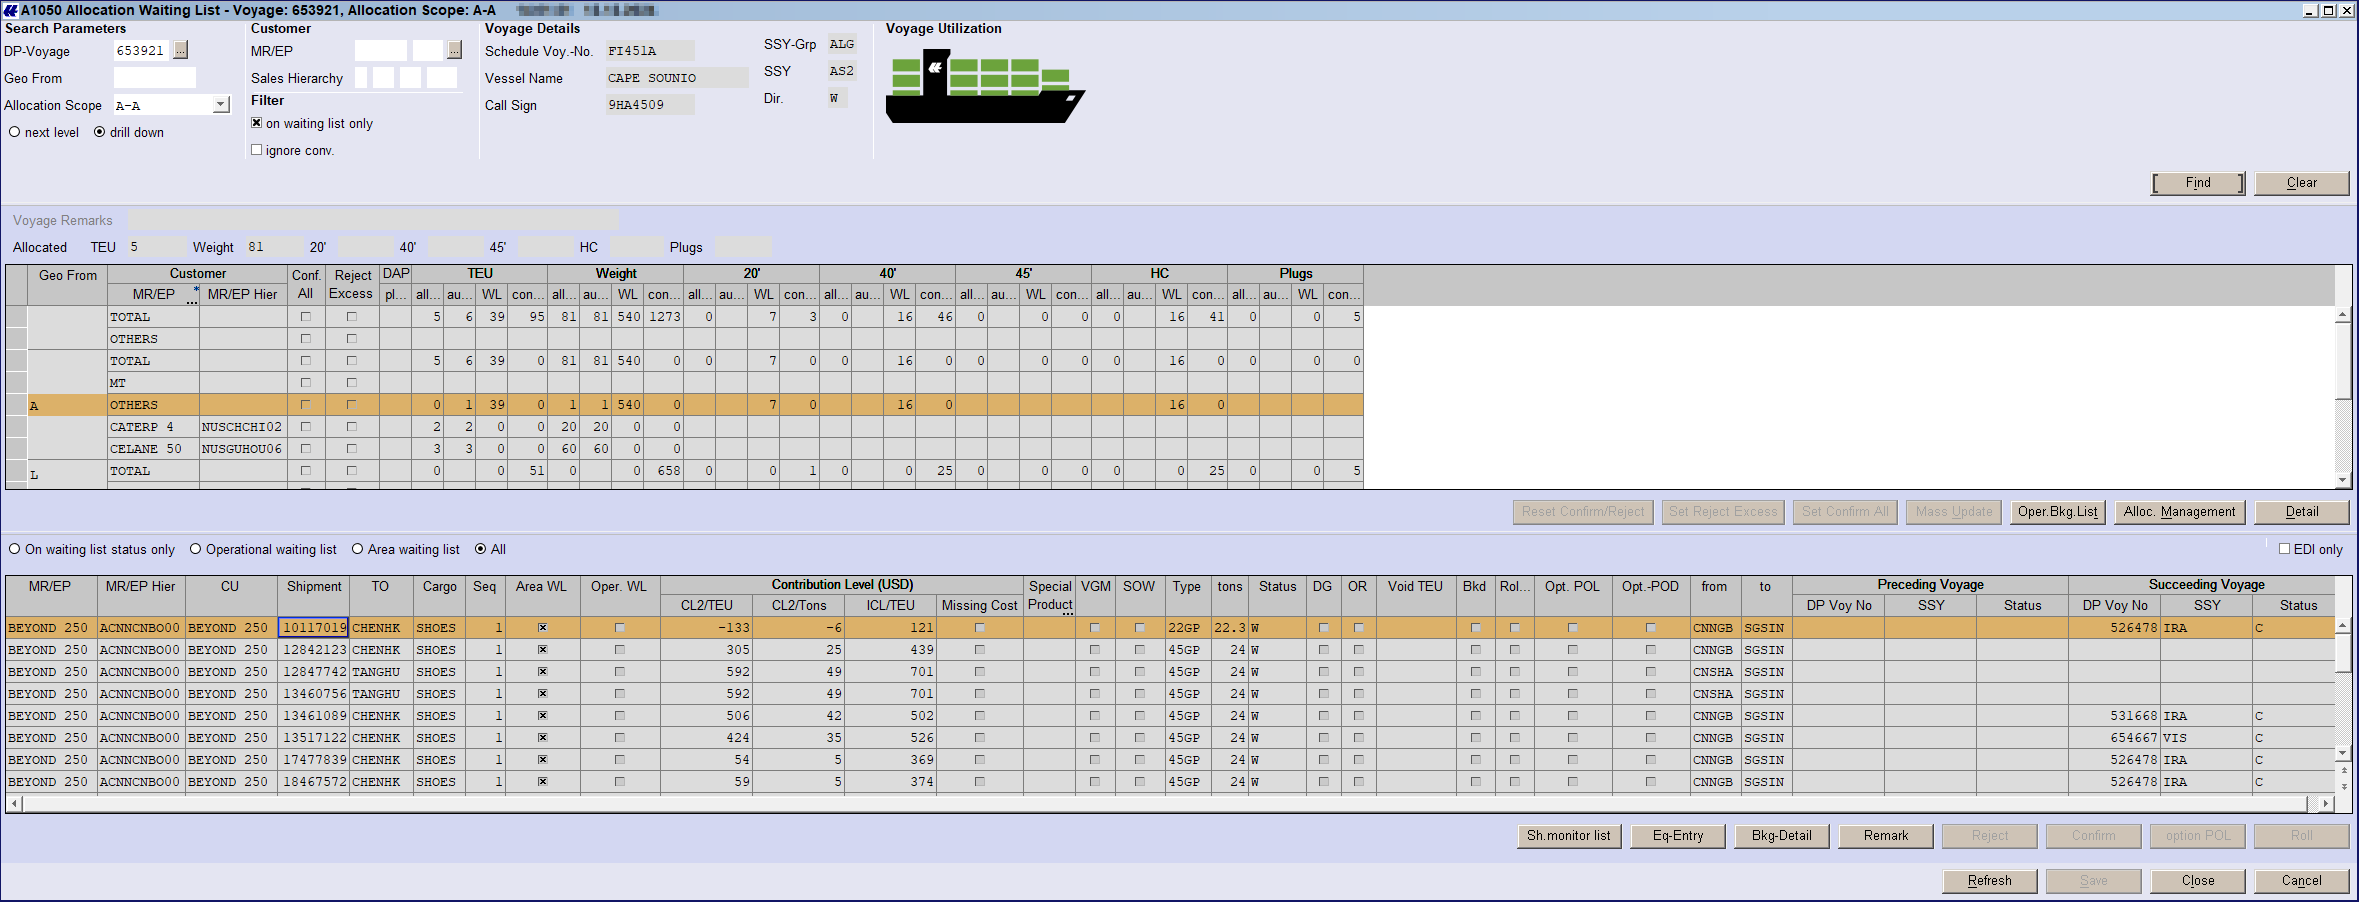
\includegraphics[width=\textwidth]{bilder/A1050.png}
    \caption
    [A1050-Screen] % Text, der im Bildverzeichnis verwendet wird
    {A1050-Screen}
    \label{fig:a1050}
\end{figure}
Auf dem Screen muss eine \gls{dpvno} und ein \enquote{Allocation-Scope} angegeben werden, wobei letzterer die Unterteilung der Fracht auf dem Schiff in verschiedene geografische Segmente beschreibt.  
Diese Segmente werden durch den Abfahrts- und Ankunftshafen definiert, wie beispielsweise Asien nach Europa.  
Danach wird eine Tabelle angezeigt, die die Herkunftsregionen angibt und in Kunden unterteilt ist.

Nach Selektion eines Kunden einer Herkunftsregion können in der unteren Tabelle die \glspl{tu} betrachtet werden, die auf der Waitinglist stehen. Diese können über die jeweilige Schaltfläche angenommen oder abgelehnt werden. Dies kann für einzelne \glspl{tu} entschieden werden. In den meisten Fällen werden aber alle \glspl{tu} einer Buchung auf einmal entschieden. Daher soll auch in dieser Arbeit das Problem nicht auf \gls{tu}, sondern auf Buchungsebene betrachtet werden. Folgend wird davon gesprochen, dass eine komplette Buchung auf der Waitinglist steht.

Nach welchen Faktoren Entscheidungen (Ablehnung, Annahme) getroffen werden, basiert auf verschiedenen Eigenschaften einer Buchung.
Viele davon sind auf dem \enquote{A1050-Screen} zu sehen.
\pagebreak

%Eine solche Tabelle können Sie weiter oben bei der geforderten und noch ausstehenden Erklärung, was eine Waitinglist ist, gerne zur Illustration benutzen, damit man sieht, wie so eine typische Waitinglist aussieht.

\begin{longtable}{lp{9cm}}
\hline
\hline
\thead{Eigenschaft} & \thead{Erklärung} \\
\hline
\endfirsthead
\hline
\thead{Eigenschaft} & \thead{Erklärung} \\
\hline
\endhead
\hline
\endfoot
\hline
\hline
\caption{Waitinglist Entscheidungsfaktoren}
\label{tab:waitinglistattr}
\endlastfoot
%Datum & Von wann ist die Entscheidung? \\
Schiffsystem\label{ref:attr_ssy} & Um welches Schiffssystem handelt es sich beim \gls{tup}? \\
Schiffsrichtung & In welche Richtung fährt das Schiff? \\
Schiffsauslastung & Wie ausgelastet ist das Schiff schon? \\
Stromanschlussverfügbarkeit & Wie viele Stromanschlüsse gibt es auf dem Schiff? \\
Stromanschlussauslastung & Wie viele Stromanschlüsse sind für das Schiff schon belegt? \\
Kunde\label{ref:attr_kunde} & Von welchem Kunden ist die Buchung? [vertraglicher Kunde, Endkunde] \\
Kundensegment & Aus welchem Segment ist der Kunde? (z.B. Autoindustrie, Chemieindustrie) \\
Bisherige Leistung & Wie profitabel war der Kunde in den vergangenen 8 Wochen? \\
Bestätigte \acrshort{teu}s & Wie viele \acrshort{teu}s sind für das Schiff schon belegt? \\
Bestätigte Tons & Wie viele Tonnen sind schon für das Schiff bestätigt? \\
Bewertung vorhanden & Ist eine wirtschaftliche Bewertung der Buchung (\gls{cl}) vorhanden? \\
\multicolumn{1}{r}{\gls{cl}2/\acrshort{teu}} & Falls eine Bewertung vorhanden ist: \gls{cl}2 / \acrshort{teu} \\
\multicolumn{1}{r}{\gls{cl}2/Tons} & Falls eine Bewertung vorhanden ist: \gls{cl}2 / Tonnen \\
\multicolumn{1}{r}{\gls{icl}/\acrshort{teu}} & Falls eine Bewertung vorhanden ist: \gls{icl} / \acrshort{teu} \\
Zusatzprodukte & Welche Zusatzprodukte hängen an der Buchung? (z.B. 50\% CO2 Kompensierung) \\
TEU & Wie viel Platz nimmt die Buchung ein? \\
Tons & Wie schwer ist die Bestellung? \\
Container Typen & Welche Containertypen sind in der Buchung? \\
Hapag Lloyd kontrolliert & Gehören die Container \gls{hl}? \\
Stromanschlüsse & Wie viele Stromanschlüsse benötigt die Buchung? \\
Gerollt zuvor & Wurde die Buchung zuvor schon mal auf ein neues Schiff verschoben (\enquote{gerollt})? \\
Gebucht zuvor & Wurde die Buchung zuvor schon mal bestellt? \\
Ladehafen & Bei welchem Hafen werden die \glspl{tu} beladen? \\
Entladehafen & Bei welchem Hafen werden die \glspl{tu} entladen? \\
Vorgangschiffssystem & Welches Schiffssystem ist vorhergehend? \\
Vorgangschiffsannahmestatus & Welchen Status hat die Buchung bei dem vorhergehenden Schiff? \\
Nachfolgeschiffssystem & Welches Schiffssystem ist nachfolgend? \\
Nachfolgeschiffsannahmestatus & Welchen Status hat die Buchung bei dem nachfolgenden Schiff?\\
\end{longtable}

%Warum wurde sich für diese Faktoren entschieden, wie wurden diese herrausgefunden

%Wie viele Shipments landen mussten in 2024 / 2025 so verarbeitet werden.
% Bezug zum Problem
Alleine im Dezember 2024 sind über $91.350$ Buchungen auf die Waitinglist gekommen \cite{BALBOA2025}.
Derzeit sind ca. 150 Mitarbeiter damit beschäftigt, alle 15 Minuten die Waitinglist zu überprüfen und falls Buchungen auf der Waitinglist vorhanden sind, zu bearbeiten. Daraus ergeben sich über 21 \glspl{fte}. \gls{fte} ist die Einheit für Vollzeitarbeitsstellen. 
Die manuelle Abarbeitung der Waitinglist bindet personelle Ressourcen und ist ein Kostenfaktor. Daher soll versucht werden, die Mitarbeiter in Zukunft so zu unterstützen, dass sie weniger Zeit für die Bearbeitung der Waitinglist aufwenden müssen.

%\todo{IW: Waitinglist erklären fehlt immernoch/ Rolle bei HL}
%Bisher haben Sie überhaupt nicht erklärt, was es mit dieser Waitinglist auf sich hat. Sie scheinen hier allgemeines Wissen beim Leser vorauszusetzen, die vielleicht jeder Mitarbeiter von Hapag-Lloyd hat. Aber das sollten Sie nicht: Setzen Sie hier null Vorkenntnisse voraus, und erklären Sie zu den Prozessen auch die verschiedenen Player darin und ihre Interessenlag.
%Welche Rolle spielt HL eigentlich? Betreiben Sie die Schiffe, sind sie der Master-Auftragnehmer, der das dann an Unterauftragnehmer verteilt, ...?


%Todo: Vielleicht bezug zu Senkung der Antwortzeitsgenze?

%%%%%%%%%%%%%%%%%%%%%%%%%%%%%%%%%%%%%%%%%%%%%
\section{Datenfluss}
\label{sec:datenfluss}
%\todo{IW: Kommentar}
%Bei jedem Training spielt die Feature Selection eine entscheidende Rolle. Daher sollten Sie Features eindeutig benennen, die einen Einfluss haben könnten und wo Sie die in den bisherigen Daten finden.

Um die Waitinglist-Entscheidung vorhersagen zu können, soll mit historischen Daten trainiert werden. Als Datenquellen gibt es bei \gls{hl} drei Möglichkeiten. Die \gls{hl} IT-Landschaft besteht grob betrachtet aus einem Altsystem (\gls{fis} 2), einem Neusystem (\gls{fis} 3) und einem Data Lake. Das Altsystem basiert auf einer monolithischen Architektur, wobei hingegen das Neusystem auf einer Mikroservice-Architektur basiert. 
\gls{hl} arbeitet konstant an der Migration vom Alt- auf das Neusystem. 
In beiden Systemen gibt es eine oder mehrere Datenbanken. 
Im monolithischen Altsystem gibt es eine große \label{ref:DB2}DB2-Instanz, ein relationales Datenbankmanagementsystem von IBM, das für die Speicherung, Verwaltung und Abfrage von strukturierten Daten entwickelt wurde \cite{IBMDb2}.   
Im Neusystem haben die einzelnen Module hingegen jeweils eigene Datenbanken.
        
Dazu gibt es aber noch den Data Lake. Ein Data Lake ist ein zentraler Speicherort, in dem große Mengen an Daten in ihrem rohen und ursprünglichen Format gespeichert werden. Im Vergleich zu den produktiven Datenbanken, die speziell für den Betrieb von Anwendungen und die Verwaltung aktueller Transaktionen optimiert sind, dient ein Data Lake hauptsächlich der Analyse und Langzeitspeicherung. Der Vorteil ist dabei, dass die produktiven Datenbanken entlastet werden, indem der Data Lake eine Plattform bereitstellt, auf der alle Daten gesammelt und für erweiterte Analysen flexibel genutzt werden können.

Der Data Lake ist die einzige Quelle für diese Untersuchung, da nur dieser die historischen Daten beinhaltet.
Er ist bei \gls{hl} in zwei Zonen eingeteilt. In die Bronze- und Silber-Zone. In der Bronze-Zone landen alle Datenänderungen unverändert. Die Silber-Zone verarbeitet die Änderungen immerhin so, dass nur noch die letzte Änderung, also der aktuelle Stand, gespeichert wird. 

Als Beispiel nehmen wir eine Tabelle mit einer ID-Spalte \enquote{ID} und einer Wert-Spalte \enquote{Wert}.

Es wird erst eine Zeile mit der ID \enquote{1} mit dem Wert \enquote{A} eingefügt und danach auf \enquote{B} geändert. 
Danach wird noch die ID \enquote{2} mit dem Wert \enquote{A} eingefügt und anschließend wieder gelöscht. 
Dies ist in der \cref{tab:zonenbsp} dargestellt.

\begin{table}[H]
    \centering
    \begin{tabular}{ccc|ccc}
         \hline
         \hline
         \multicolumn{3}{c|}{\thead{\textbf{Bronze-Zone}}}&  \multicolumn{3}{c}{\textbf{Silber-Zone}}\\
         \hline
         \thead{ID}&  Wert&  Letzte Aktion&  ID&  Wert& Letzte Aktion\\
         \hline
         1&  A&  Einfügen&  1&  B& Ändern\\
         1&  B&  Ändern&  2&  A& Löschen\\
         2&  A&  Einfügen&  &  & \\
         2&  A&  Löschen&  &  & \\
         \hline
         \hline
    \end{tabular}
    \caption{Beispiel: Bronze- und Silber-Zonentabelle}
    \label{tab:zonenbsp}
\end{table}
In der Bronze-Zone sieht man nun, dass alle Änderungen als einzelne Zeilen mit ihrer Aktion hinterlegt wurden. In der Silber-Zone hingegen wird immer nur der aktuelle Stand gespeichert. Der einzige Unterschied zwischen der Silber-Zone und der produktiven Datenbank ist, dass gelöschte Einträge immer noch gefunden werden können. Gelöschte Einträge sind aber in der Silber-Zone über die \enquote{letzte Aktion}-Spalte als gelöscht markiert.

Daher ist die Datenquelle dieser Arbeit der Data Lake.
%\todo{IW: Implementations detail}
%Mir scheint die Sache, was sich in Bronze, Silber oder im Data Lake befindet, ein ziemliches Implementierungsdetails zu sein, das Sie natürlich auch für Ihre Lösung berücksichtigen müssen.
%An dieser Stelle müssen Sie den Leser aber erst mal informieren, was für eine Art Daten Sie überhaupt korrelieren, um etwas zu lernen.


%%%%%%%%%%%%%%%%%%%%%%%%%%%%%%%%%%%%%%%%%%%%%
\subsection{Prozess}


Im Folgenden wird darauf eingegangen, wie sich Daten zwischen den verschiedenen Systemen verteilen und wie sie letztlich in den Data Lake gelangen. Dieser Prozess ist nicht nur für den Aufbau eines Data Lakes relevant, sondern auch für die Synchronisation von Daten zwischen unterschiedlichen Systemen. 

Um diese Aufgabe zu bewältigen, wird bei \gls{hl} das Werkzeug \enquote{Qlik Replicate} eingesetzt. \enquote{Qlik Replicate} ist ein Tool zur Datenreplikation und -integration, welches Daten zwischen verschiedenen Quellen, wie Datenbanken und Data Warehouses, synchronisiert \cite{QlikReplicate}. Bei \gls{hl} wird es verwendet, um Änderungen aus einer DB2-Datenbank in \gls{aws} S3 Buckets zu replizieren. S3-Buckets sind Speichercontainer in \gls{aws}, die Daten sicher und skalierbar speichern und organisieren \cite{AWS_S3_Buckets}. Zudem handelt es sich hierbei um eine günstige Variante, Daten in \gls{aws} zu speichern. 

\begin{figure}[H]
    \centering
    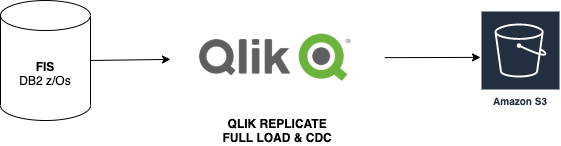
\includegraphics[width=0.5\textwidth]{Thesis/bilder/qlikdiagram.drawio.png}
    \caption
    [Replikationsprozess Visualisierung]
    {Replikationsprozess Visualisierung}
    \label{fig:qlikrep}
\end{figure}

Neben der Replikation in S3-Buckets wird \enquote{Qlik Replicate} auch genutzt, um Datenbankänderungen, sogenannte Change Data Capture (CDC)-Events, in Kafka Topics zu schreiben. Diese Kafka Topics ermöglichen es den einzelnen Modulen des Neusystems, die benötigten Daten eigenständig und gezielt zu verarbeiten.

Die Daten werden also bei \gls{hl} in verschiedenen Systemen verteilt. 
Um in den verschiedenen Systemen zu suchen, wo welche Daten liegen, kann das Tool \enquote{Collibra} verwendet werden.
Dies ist eine Datenkatalogplattform, auf der bei \gls{hl} automatisiert die Datenstruktur hinterlegt wird. 
Das funktioniert ähnlich wie bei den S3 Buckets, nur wird nicht \enquote{Qlik Replicate} verwendet, um die Daten zu übertragen. Es werden die Schemadaten aus den einzelnen Systemen direkt zu \enquote{Collibra} übertragen. 

 
\subsection{Databricks}
\label{sec:databricks}
Databricks ist eine cloudbasierte Plattform, die auf Apache Spark, einem Framework für verteilte Datenverarbeitung, basiert. Sie wurde entwickelt, um große Datenmengen zu verarbeiten, zu analysieren und zu verwalten, und bietet eine einheitliche Umgebung für Daten-Engineering, Datenanalyse und \gls{ml} \cite{DatabricksSpark}. 
Die Plattform ermöglicht die Verarbeitung von Daten aus verschiedenen Quellen, einschließlich relationaler Datenbanken und Cloud-Speicher.

Bei \gls{hl} dienen die \gls{aws} S3-Buckets als zentrale Datenquelle für Databricks. 
Databricks fungiert in diesem Kontext als Schnittstelle zum Data Lake, mit der in dieser Arbeit Daten zur Verwendung aggregiert werden. Innerhalb der Plattform wurden alle wesentlichen Implementierungen durchgeführt, was sie zur Hauptarbeitsumgebung im Rahmen dieser Arbeit macht.

Ein zentrales Merkmal von Databricks sind interaktive Notebooks, die als Entwicklungs- und Kollaborationsumgebung dienen. Ein Notebook ist eine Umgebung, in der Code geschrieben und ausgeführt, Daten analysiert sowie Ergebnisse visualisiert werden können. Notebooks unterstützen mehrere Programmiersprachen wie Python, SQL, Scala und R. Sie bieten integrierte Visualisierungen und ermöglichen eine einfache Zusammenarbeit in Echtzeit \cite{DatabricksNotebooks}. In dieser Arbeit war dies die zentrale Arbeitsstelle und wurde genutzt, um Daten zu aggregieren, zu analysieren und Modelle für maschinelles Lernen zu trainieren.

Für die Ausführung der Notebooks verwendet Databricks sogenannte Compute-Cluster. Dabei handelt es sich um virtuelle Rechner in der Cloud, die speziell für die parallele Verarbeitung von Daten mittels Apache Spark konfiguriert sind. Die Arbeit in den Notebooks ermöglicht einen schnellen Zugriff auf die bereits in Databricks verfügbaren Daten. Dadurch wird sichergestellt, dass die lokalen Ressourcen eines Arbeitsplatzes nicht performant sein müssen, da alle rechenintensiven Prozesse auf den Cloud-Clustern ausgeführt werden.

Bei \gls{hl} werden \gls{aws} EC2-Instanzen für die Compute-Cluster verwendet. 
Dabei kann bei jedem Compute-Cluster selbst konfiguriert werden, was für eine oder mehrere EC2-Instanzen betrieben und verwendet werden. 
Diese Auswahl entscheidet, ob keine/eine/mehrere \glspl{gpu} verwendet werden sollen, sowie wie viel Leistung für die Ausführung eines Notebooks zur Verfügung steht.
